\PassOptionsToPackage{unicode=true}{hyperref} % options for packages loaded elsewhere
\PassOptionsToPackage{hyphens}{url}
\PassOptionsToPackage{dvipsnames,svgnames*,x11names*}{xcolor}
%
\documentclass[10pt,ignorenonframetext,serif,onlymath]{beamer}
\setbeamertemplate{caption}[numbered]
\setbeamertemplate{caption label separator}{: }
\setbeamercolor{caption name}{fg=normal text.fg}
\beamertemplatenavigationsymbolsempty
\usepackage{lmodern}
\usepackage{amssymb,amsmath}
\usepackage{ifxetex,ifluatex}
\usepackage{fixltx2e} % provides \textsubscript
\ifnum 0\ifxetex 1\fi\ifluatex 1\fi=0 % if pdftex
  \usepackage[T1]{fontenc}
  \usepackage[utf8]{inputenc}
  \usepackage{textcomp} % provides euro and other symbols
\else % if luatex or xelatex
  \usepackage{unicode-math}
  \defaultfontfeatures{Ligatures=TeX,Scale=MatchLowercase}
\fi
% use upquote if available, for straight quotes in verbatim environments
\IfFileExists{upquote.sty}{\usepackage{upquote}}{}
% use microtype if available
\IfFileExists{microtype.sty}{%
\usepackage[]{microtype}
\UseMicrotypeSet[protrusion]{basicmath} % disable protrusion for tt fonts
}{}
\IfFileExists{parskip.sty}{%
\usepackage{parskip}
}{% else
\setlength{\parindent}{0pt}
\setlength{\parskip}{6pt plus 2pt minus 1pt}
}
\usepackage{xcolor}
\usepackage{hyperref}
\hypersetup{
            pdftitle={Cutting-plane Method and the Amazing Oracles (II)},
            pdfauthor={Wai-Shing Luk},
            colorlinks=true,
            linkcolor=Maroon,
            citecolor=Blue,
            urlcolor=Blue,
            breaklinks=true}
\urlstyle{same}  % don't use monospace font for urls
\newif\ifbibliography
\usepackage{color}
\usepackage{fancyvrb}
\newcommand{\VerbBar}{|}
\newcommand{\VERB}{\Verb[commandchars=\\\{\}]}
\DefineVerbatimEnvironment{Highlighting}{Verbatim}{commandchars=\\\{\}}
% Add ',fontsize=\small' for more characters per line
\newenvironment{Shaded}{}{}
\newcommand{\AlertTok}[1]{\textcolor[rgb]{1.00,0.00,0.00}{\textbf{#1}}}
\newcommand{\AnnotationTok}[1]{\textcolor[rgb]{0.38,0.63,0.69}{\textbf{\textit{#1}}}}
\newcommand{\AttributeTok}[1]{\textcolor[rgb]{0.49,0.56,0.16}{#1}}
\newcommand{\BaseNTok}[1]{\textcolor[rgb]{0.25,0.63,0.44}{#1}}
\newcommand{\BuiltInTok}[1]{#1}
\newcommand{\CharTok}[1]{\textcolor[rgb]{0.25,0.44,0.63}{#1}}
\newcommand{\CommentTok}[1]{\textcolor[rgb]{0.38,0.63,0.69}{\textit{#1}}}
\newcommand{\CommentVarTok}[1]{\textcolor[rgb]{0.38,0.63,0.69}{\textbf{\textit{#1}}}}
\newcommand{\ConstantTok}[1]{\textcolor[rgb]{0.53,0.00,0.00}{#1}}
\newcommand{\ControlFlowTok}[1]{\textcolor[rgb]{0.00,0.44,0.13}{\textbf{#1}}}
\newcommand{\DataTypeTok}[1]{\textcolor[rgb]{0.56,0.13,0.00}{#1}}
\newcommand{\DecValTok}[1]{\textcolor[rgb]{0.25,0.63,0.44}{#1}}
\newcommand{\DocumentationTok}[1]{\textcolor[rgb]{0.73,0.13,0.13}{\textit{#1}}}
\newcommand{\ErrorTok}[1]{\textcolor[rgb]{1.00,0.00,0.00}{\textbf{#1}}}
\newcommand{\ExtensionTok}[1]{#1}
\newcommand{\FloatTok}[1]{\textcolor[rgb]{0.25,0.63,0.44}{#1}}
\newcommand{\FunctionTok}[1]{\textcolor[rgb]{0.02,0.16,0.49}{#1}}
\newcommand{\ImportTok}[1]{#1}
\newcommand{\InformationTok}[1]{\textcolor[rgb]{0.38,0.63,0.69}{\textbf{\textit{#1}}}}
\newcommand{\KeywordTok}[1]{\textcolor[rgb]{0.00,0.44,0.13}{\textbf{#1}}}
\newcommand{\NormalTok}[1]{#1}
\newcommand{\OperatorTok}[1]{\textcolor[rgb]{0.40,0.40,0.40}{#1}}
\newcommand{\OtherTok}[1]{\textcolor[rgb]{0.00,0.44,0.13}{#1}}
\newcommand{\PreprocessorTok}[1]{\textcolor[rgb]{0.74,0.48,0.00}{#1}}
\newcommand{\RegionMarkerTok}[1]{#1}
\newcommand{\SpecialCharTok}[1]{\textcolor[rgb]{0.25,0.44,0.63}{#1}}
\newcommand{\SpecialStringTok}[1]{\textcolor[rgb]{0.73,0.40,0.53}{#1}}
\newcommand{\StringTok}[1]{\textcolor[rgb]{0.25,0.44,0.63}{#1}}
\newcommand{\VariableTok}[1]{\textcolor[rgb]{0.10,0.09,0.49}{#1}}
\newcommand{\VerbatimStringTok}[1]{\textcolor[rgb]{0.25,0.44,0.63}{#1}}
\newcommand{\WarningTok}[1]{\textcolor[rgb]{0.38,0.63,0.69}{\textbf{\textit{#1}}}}
\usepackage{graphicx,grffile}
\makeatletter
\def\maxwidth{\ifdim\Gin@nat@width>\linewidth\linewidth\else\Gin@nat@width\fi}
\def\maxheight{\ifdim\Gin@nat@height>\textheight\textheight\else\Gin@nat@height\fi}
\makeatother
% Scale images if necessary, so that they will not overflow the page
% margins by default, and it is still possible to overwrite the defaults
% using explicit options in \includegraphics[width, height, ...]{}
\setkeys{Gin}{width=\maxwidth,height=\maxheight,keepaspectratio}
% Prevent slide breaks in the middle of a paragraph:
\widowpenalties 1 10000
\raggedbottom
\setbeamertemplate{part page}{
\centering
\begin{beamercolorbox}[sep=16pt,center]{part title}
  \usebeamerfont{part title}\insertpart\par
\end{beamercolorbox}
}
\setbeamertemplate{section page}{
\centering
\begin{beamercolorbox}[sep=12pt,center]{part title}
  \usebeamerfont{section title}\insertsection\par
\end{beamercolorbox}
}
\setbeamertemplate{subsection page}{
\centering
\begin{beamercolorbox}[sep=8pt,center]{part title}
  \usebeamerfont{subsection title}\insertsubsection\par
\end{beamercolorbox}
}
\AtBeginPart{
  \frame{\partpage}
}
\AtBeginSection{
  \ifbibliography
  \else
    \frame{\sectionpage}
  \fi
}
\AtBeginSubsection{
  \frame{\subsectionpage}
}
\setlength{\emergencystretch}{3em}  % prevent overfull lines
\providecommand{\tightlist}{%
  \setlength{\itemsep}{0pt}\setlength{\parskip}{0pt}}
\setcounter{secnumdepth}{0}

% set default figure placement to htbp
\makeatletter
\def\fps@figure{htbp}
\makeatother

\usetheme{default}
\usepackage{tikz,pgf,pgfplots}
\usetikzlibrary{arrows}
\definecolor{qqqqff}{rgb}{0.,0.,1.}
\newcommand{\columnsbegin}{\begin{columns}}
\newcommand{\columnsend}{\end{columns}}
\newcommand{\col}[1]{\column{#1}}
\pgfdeclareimage[height=0.5cm]{fudan-logo}{fudan-logo.jpg}
\logo{\pgfuseimage{fudan-logo}}

\title{Cutting-plane Method and the Amazing Oracles (II)}
\author{Wai-Shing Luk}
\providecommand{\institute}[1]{}
\institute{Fudan University}
\date{\today}

\begin{document}
\frame{\titlepage}

\begin{frame}
\tableofcontents[hideallsubsections]
\end{frame}
\hypertarget{ellipsoid-method-revisited}{%
\section{Ellipsoid Method Revisited}\label{ellipsoid-method-revisited}}

\begin{frame}{Basic Ellipsoid Method}
\protect\hypertarget{basic-ellipsoid-method}{}

\begin{itemize}
\tightlist
\item
  An ellipsoid \(\mathcal{E}(x_c, P)\) is specified as a set
  \[\{x \mid (x-x_c)P^{-1}(x-x_c) \leq 1 \},\] where \(x_c\) is the
  center of the ellipsoid.
\end{itemize}

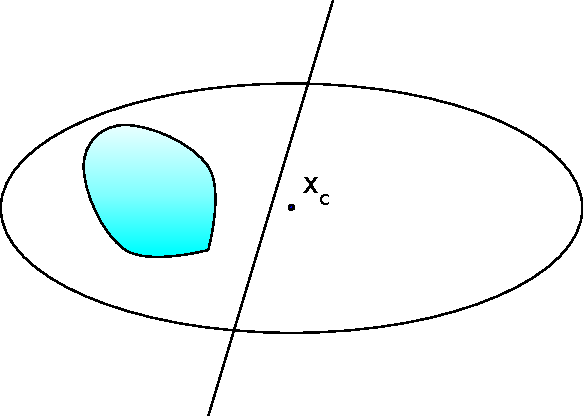
\includegraphics[width=0.6\textwidth,height=\textheight]{ellipsoid.files/ellipsoid.pdf}

\end{frame}

\begin{frame}[fragile]{Python code}
\protect\hypertarget{python-code}{}

\begin{Shaded}
\begin{Highlighting}[]
\ImportTok{import}\NormalTok{ numpy }\ImportTok{as}\NormalTok{ np}

\KeywordTok{class}\NormalTok{ ell:}
    \KeywordTok{def} \FunctionTok{__init__}\NormalTok{(}\VariableTok{self}\NormalTok{, val, x):}
        \CommentTok{'''ell = \{ x | (x - xc)' * P^-1 * (x - xc) <= 1 \}'''}
\NormalTok{        n }\OperatorTok{=} \BuiltInTok{len}\NormalTok{(x)}
        \ControlFlowTok{if}\NormalTok{ np.isscalar(val):}
            \VariableTok{self}\NormalTok{.P }\OperatorTok{=}\NormalTok{ val }\OperatorTok{*}\NormalTok{ np.identity(n)}
        \ControlFlowTok{else}\NormalTok{:}
            \VariableTok{self}\NormalTok{.P }\OperatorTok{=}\NormalTok{ np.diag(val)}
        \VariableTok{self}\NormalTok{.xc }\OperatorTok{=}\NormalTok{ np.array(x)}
        \VariableTok{self}\NormalTok{.c1 }\OperatorTok{=} \BuiltInTok{float}\NormalTok{(n}\OperatorTok{*}\NormalTok{n)}\OperatorTok{/}\NormalTok{(n}\OperatorTok{*}\NormalTok{n}\FloatTok{-1.}\NormalTok{)}

    \KeywordTok{def}\NormalTok{ update_core(}\VariableTok{self}\NormalTok{, calc_ell, cut):...}
    \KeywordTok{def}\NormalTok{ calc_cc(}\VariableTok{self}\NormalTok{, g):...}
    \KeywordTok{def}\NormalTok{ calc_dc(}\VariableTok{self}\NormalTok{, cut):...}
    \KeywordTok{def}\NormalTok{ calc_ll(}\VariableTok{self}\NormalTok{, cut):...}
\end{Highlighting}
\end{Shaded}

\end{frame}

\begin{frame}{Updating the ellipsoid (deep-cut)}
\protect\hypertarget{updating-the-ellipsoid-deep-cut}{}

\begin{itemize}
\tightlist
\item
  Calculation of minimum volume ellipsoid covering:
  \[\mathcal{E} \cap \{z \mid g^\top (z - x_c) + h \leq 0 \}\]
\item
  Let \(\tilde{g} = P\,g\), \(\tau^2 = g^\top P g\).
\item
  If \(n \cdot h < -\tau\) (shallow cut), no smaller ellipsoid can be
  found.
\item
  If \(h > \tau\), intersection is empty.
\item
  Otherwise, \[x_c^+ = x_c - \frac{\rho}{ \tau^2 } \tilde{g}, \qquad
  P^+ = {\color{orange}\delta\cdot}\left(P - \frac{\sigma}{ \tau^2 } \tilde{g}\tilde{g}^\top\right)\]
\end{itemize}

where \[\rho = \frac{ {\color{red}\tau}+nh}{n+1}, \qquad
  \sigma = \frac{2\rho}{ {\color{red}\tau}+h}, \qquad
  \delta = \frac{n^2(\tau^2 - h^2)}{(n^2 - 1)\tau^2}\]

\end{frame}

\begin{frame}{Updating the ellipsoid (cont’d)}
\protect\hypertarget{updating-the-ellipsoid-contd}{}

\begin{itemize}
\tightlist
\item
  Even better, split \(P\) into two variables \(\kappa \cdot Q\)
\item
  Let \(\tilde{g} = Q \cdot g\), \(\omega = g^\top\tilde{g}\),
  \(\tau = \sqrt{\kappa\cdot\omega}\).
  \[x_c^+ = x_c - \frac{\rho}{\omega} \tilde{g}, \qquad
  Q^+ = Q - \frac{\sigma}{\omega} \tilde{g}\tilde{g}^\top, \qquad
  \kappa^+ =  \delta\cdot\kappa
   \]
\item
  Reduce \(n^2\) multiplications per iteration.
\item
  Note:

  \begin{itemize}
  \tightlist
  \item
    The determinant of \(Q\) decreases monotonically.
  \item
    The range of \(\delta\) is \((0, \frac{n^2}{n^2 - 1})\)
  \end{itemize}
\end{itemize}

\end{frame}

\begin{frame}[fragile]{Python code (updating)}
\protect\hypertarget{python-code-updating}{}

\begin{Shaded}
\begin{Highlighting}[]
\KeywordTok{def}\NormalTok{ update_core(}\VariableTok{self}\NormalTok{, calc_ell, cut):}
\NormalTok{    g, beta }\OperatorTok{=}\NormalTok{ cut}
\NormalTok{    Qg }\OperatorTok{=} \VariableTok{self}\NormalTok{.Q.dot(g)}
\NormalTok{    omega }\OperatorTok{=}\NormalTok{ g.dot(Qg)}
\NormalTok{    tsq }\OperatorTok{=} \VariableTok{self}\NormalTok{.kappa }\OperatorTok{*}\NormalTok{ omega}
    \ControlFlowTok{if}\NormalTok{ tsq }\OperatorTok{<=} \FloatTok{0.}\NormalTok{:}
        \ControlFlowTok{return} \DecValTok{4}\NormalTok{, }\FloatTok{0.}
\NormalTok{    status, params }\OperatorTok{=}\NormalTok{ calc_ell(beta, tsq)}
    \ControlFlowTok{if}\NormalTok{ status }\OperatorTok{!=} \DecValTok{0}\NormalTok{:}
        \ControlFlowTok{return}\NormalTok{ status, tsq}
\NormalTok{    rho, sigma, delta }\OperatorTok{=}\NormalTok{ params}
    \VariableTok{self}\NormalTok{._xc }\OperatorTok{-=}\NormalTok{ (rho }\OperatorTok{/}\NormalTok{ omega) }\OperatorTok{*}\NormalTok{ Qg}
    \VariableTok{self}\NormalTok{.Q }\OperatorTok{-=}\NormalTok{ (sigma }\OperatorTok{/}\NormalTok{ omega) }\OperatorTok{*}\NormalTok{ np.outer(Qg, Qg)}
    \VariableTok{self}\NormalTok{.kappa }\OperatorTok{*=}\NormalTok{ delta}
    \ControlFlowTok{return}\NormalTok{ status, tsq}
\end{Highlighting}
\end{Shaded}

\end{frame}

\begin{frame}[fragile]{Python code (deep cut)}
\protect\hypertarget{python-code-deep-cut}{}

\begin{Shaded}
\begin{Highlighting}[]
\KeywordTok{def}\NormalTok{ calc_dc(}\VariableTok{self}\NormalTok{, beta, tsq):}
    \CommentTok{'''deep cut'''}
\NormalTok{    tau }\OperatorTok{=}\NormalTok{ math.sqrt(tsq)}
    \ControlFlowTok{if}\NormalTok{ beta }\OperatorTok{>}\NormalTok{ tau:}
        \ControlFlowTok{return} \DecValTok{1}\NormalTok{, }\VariableTok{None}    \CommentTok{# no sol'n}
    \ControlFlowTok{if}\NormalTok{ beta }\OperatorTok{==} \FloatTok{0.}\NormalTok{:}
        \ControlFlowTok{return} \VariableTok{self}\NormalTok{.calc_cc(tau)}
\NormalTok{    n }\OperatorTok{=} \VariableTok{self}\NormalTok{._n}
\NormalTok{    gamma }\OperatorTok{=}\NormalTok{ tau }\OperatorTok{+}\NormalTok{ n}\OperatorTok{*}\NormalTok{beta}
    \ControlFlowTok{if}\NormalTok{ gamma }\OperatorTok{<} \FloatTok{0.}\NormalTok{:}
        \ControlFlowTok{return} \DecValTok{3}\NormalTok{, }\VariableTok{None}  \CommentTok{# no effect}
\NormalTok{    rho }\OperatorTok{=}\NormalTok{ gamma}\OperatorTok{/}\NormalTok{(n }\OperatorTok{+} \DecValTok{1}\NormalTok{)}
\NormalTok{    sigma }\OperatorTok{=} \FloatTok{2.}\OperatorTok{*}\NormalTok{rho}\OperatorTok{/}\NormalTok{(tau }\OperatorTok{+}\NormalTok{ beta)}
\NormalTok{    delta }\OperatorTok{=} \VariableTok{self}\NormalTok{.c1}\OperatorTok{*}\NormalTok{(tsq }\OperatorTok{-}\NormalTok{ beta}\OperatorTok{**}\DecValTok{2}\NormalTok{)}\OperatorTok{/}\NormalTok{tsq}
    \ControlFlowTok{return} \DecValTok{0}\NormalTok{, (rho, sigma, delta)}
\end{Highlighting}
\end{Shaded}

\end{frame}

\begin{frame}{Central Cut}
\protect\hypertarget{central-cut}{}

\begin{itemize}
\tightlist
\item
  A Special case of deep cut when \(\beta = 0\)
\item
  Deserve a separate implement because it is much simplier.
\item
  Let \(\tilde{g} = Q\,g\), \(\tau = \sqrt{\kappa\cdot\omega}\),
\end{itemize}

\[\rho = {\tau \over n+1}, \qquad
  \sigma = {2 \over n+1}, \qquad
  \delta = {n^2 \over n^2 - 1}\]

\end{frame}

\begin{frame}[fragile]{Python code (deep cut)}
\protect\hypertarget{python-code-deep-cut-1}{}

\begin{Shaded}
\begin{Highlighting}[]
\KeywordTok{def}\NormalTok{ calc_cc(}\VariableTok{self}\NormalTok{, tau):}
    \CommentTok{'''central cut'''}
\NormalTok{    np1 }\OperatorTok{=} \VariableTok{self}\NormalTok{._n }\OperatorTok{+} \DecValTok{1}
\NormalTok{    sigma }\OperatorTok{=} \FloatTok{2.} \OperatorTok{/}\NormalTok{ np1}
\NormalTok{    rho }\OperatorTok{=}\NormalTok{ tau }\OperatorTok{/}\NormalTok{ np1}
\NormalTok{    delta }\OperatorTok{=} \VariableTok{self}\NormalTok{.c1}
    \ControlFlowTok{return} \DecValTok{0}\NormalTok{, (rho, sigma, delta)}
\end{Highlighting}
\end{Shaded}

\end{frame}

\begin{frame}{Parallel Cuts}
\protect\hypertarget{parallel-cuts}{}

\begin{itemize}
\item
  Oracle returns a pair of cuts instead of just one.
\item
  The pair of cuts is given by \(g\) and \((\beta_1, \beta_2)\) such
  that: \[\begin{array}{l}
  g^\top (x - x_c) + \beta_1 \leq 0,  \\
  g^\top (x - x_c) + \beta_2 \geq 0,
  \end{array}\] for all \(x \in \mathcal{K}\).
\item
  Only linear inequality constraint can produce such parallel cut:
  \[ l \leq a^\top x + b \leq u, \qquad L \preceq F(x) \preceq U \]
\item
  Usually provide faster convergence.
\end{itemize}

\end{frame}

\begin{frame}{Parallel Cuts}
\protect\hypertarget{parallel-cuts-1}{}

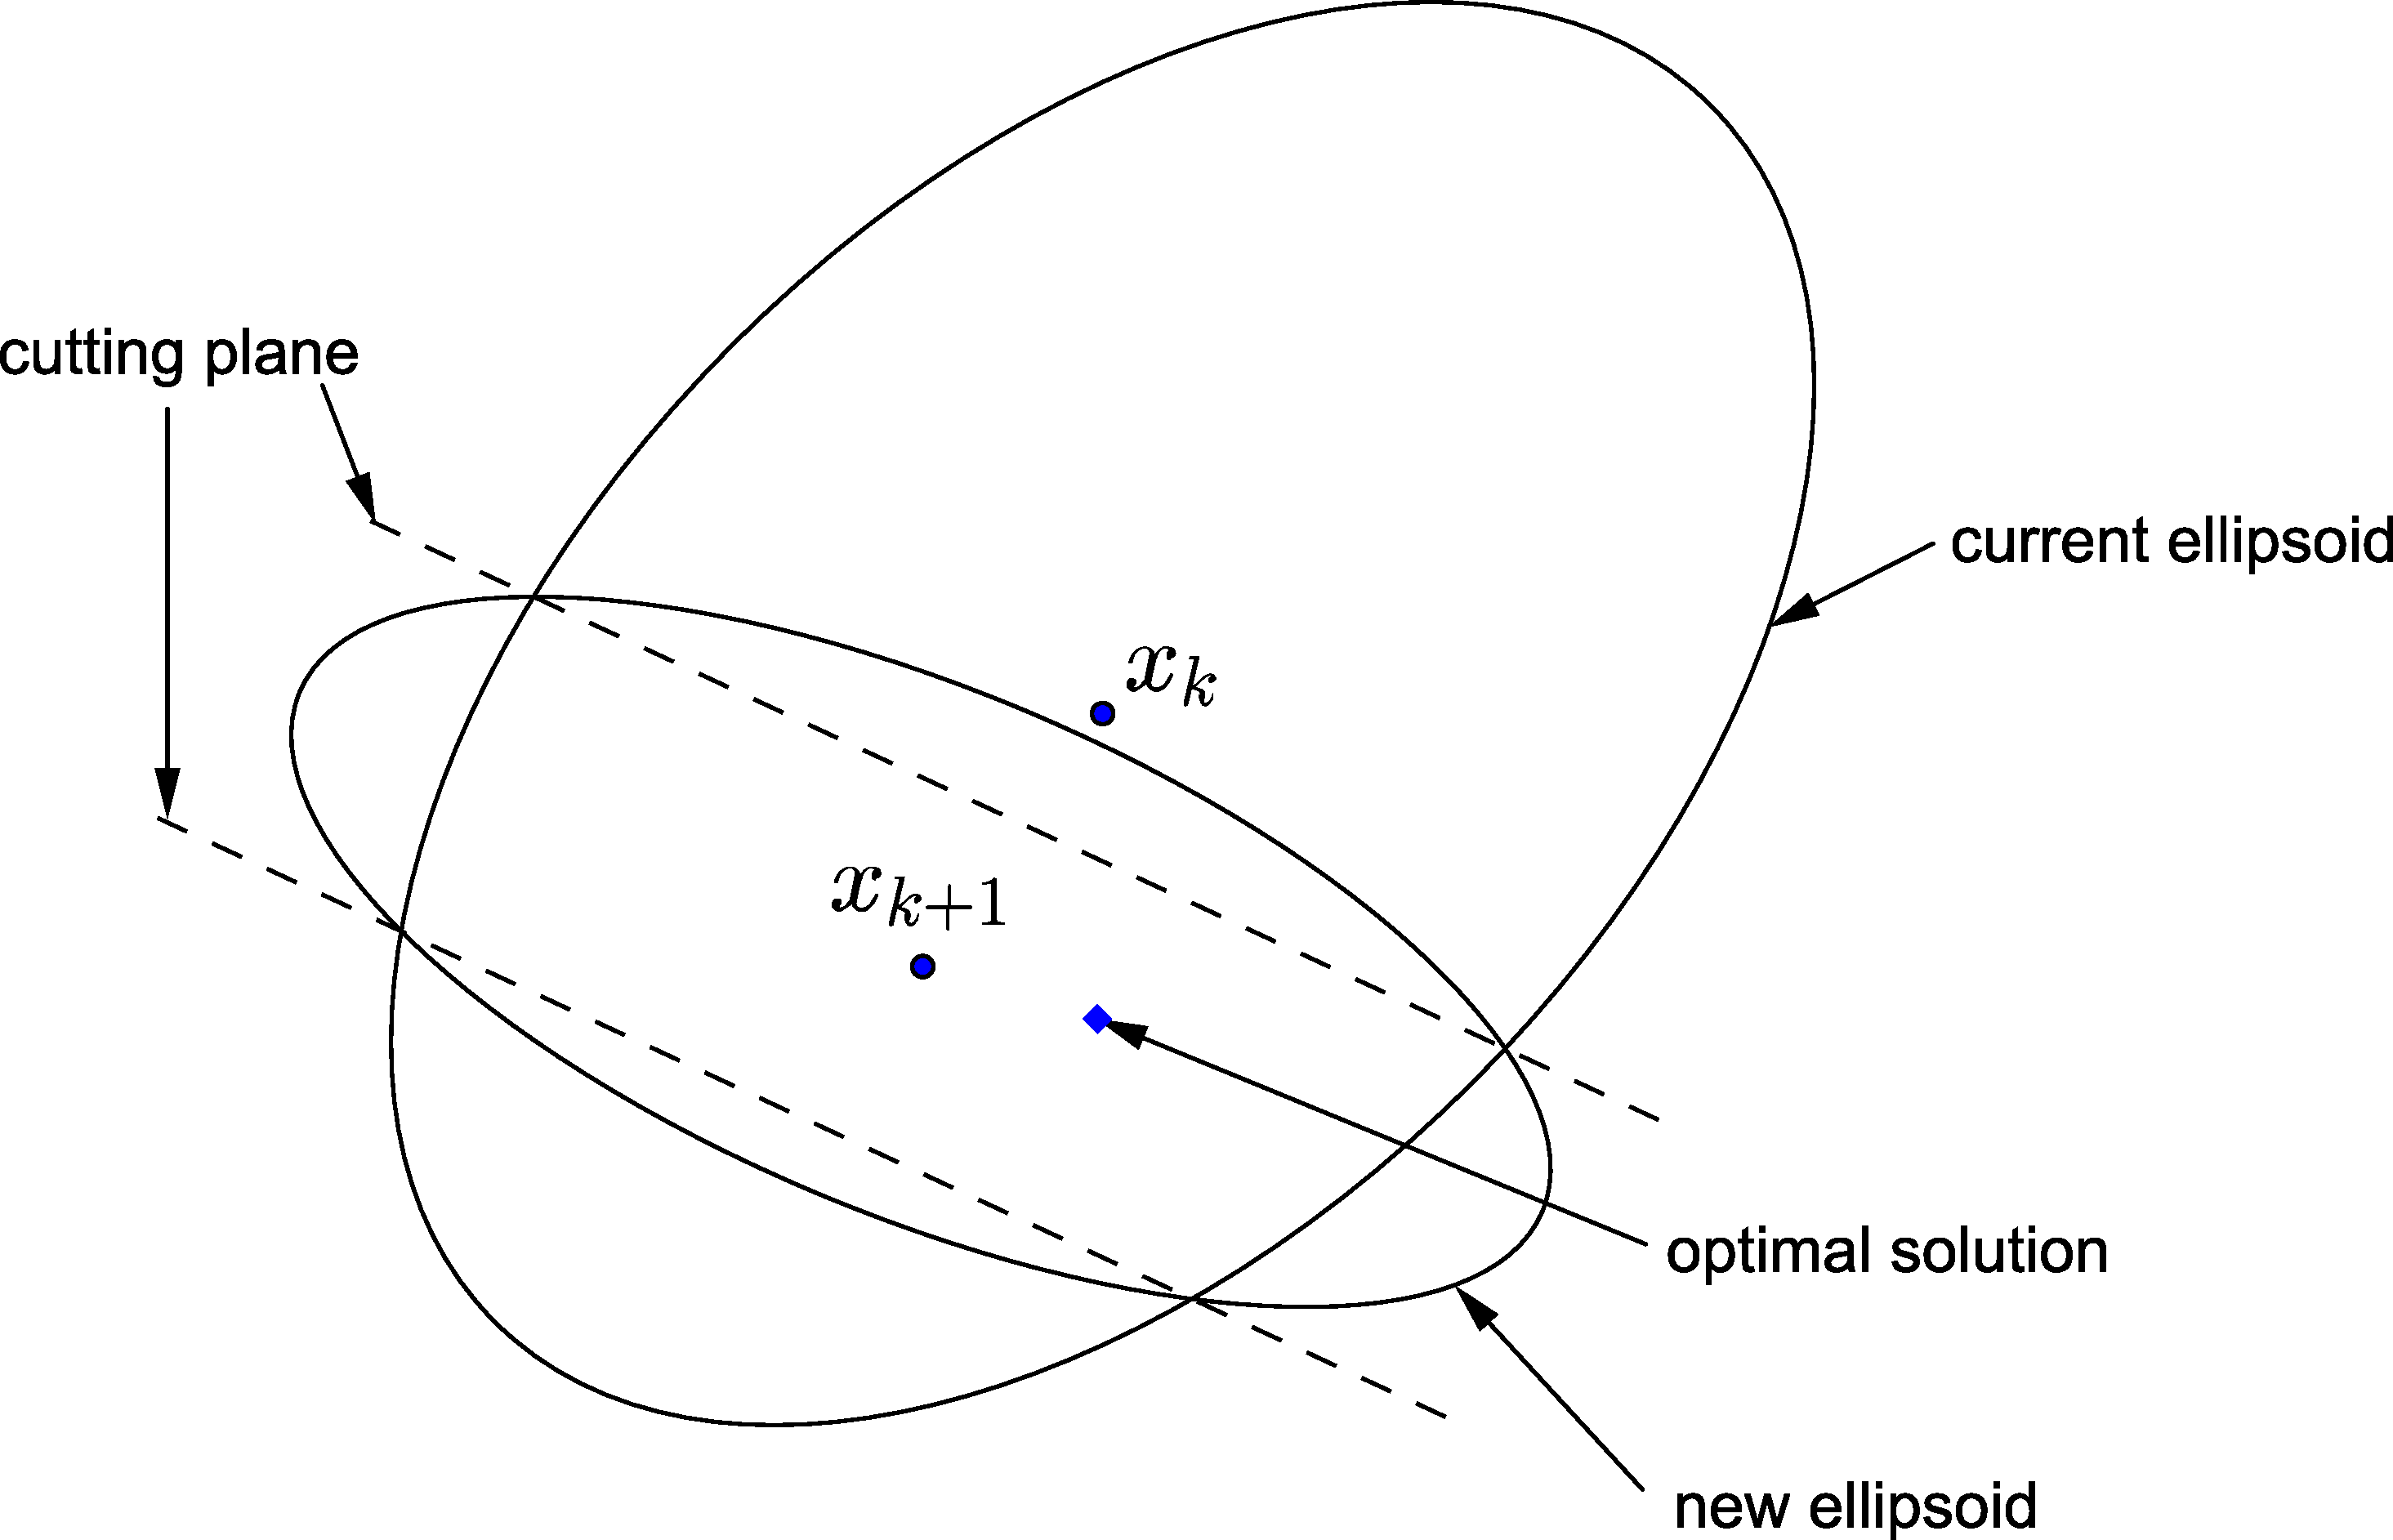
\includegraphics{ellipsoid.files/parallel_cut.pdf}

\end{frame}

\begin{frame}{Updating the ellipsoid}
\protect\hypertarget{updating-the-ellipsoid}{}

\begin{itemize}
\item
  Let \(\tilde{g} = Q\,g\), \(\tau^2 = \kappa\cdot\omega\).
\item
  If \(\beta_1 > \beta_2\), intersection is empty.
\item
  If \(\beta_1 \beta_2 < -\tau^2/n\), no smaller ellipsoid can be found.
\item
  If \(\beta_2^2 > \tau^2\), it reduces to deep-cut with
  \(\alpha = \alpha_1\).
\item
  Otherwise, \[x_c^+ = x_c - \frac{\rho}{\omega} \tilde{g}, \qquad
  Q^+ = Q - \frac{\sigma}{\omega} \tilde{g}\tilde{g}^\top, \qquad
  \kappa^+ =  \delta \kappa
   \]

  where \[\begin{array}{lll}
    \bar{\beta} &=& (\beta_1 + \beta_2)/2 \\
    \xi^2 &=& (\tau^2 - \beta_1^2)(\tau^2 - \beta_2^2) + (n(\beta_2 - \beta_1)\bar{\beta})^2, \\
    \sigma &=& (n + (\tau^2 - \beta_1\beta_2 - \xi)/(2\bar{\beta}^2)) / (n + 1), \\
    \rho &=& \bar{\beta}\cdot\sigma, \\
    \delta &=& (n^2/(n^2-1)) (\tau^2 - (\beta_1^2 + \beta_2^2)/2 + \xi/n) / \tau^2
   \end{array}\]
\end{itemize}

\end{frame}

\begin{frame}[fragile]{Python code (parallel cut)}
\protect\hypertarget{python-code-parallel-cut}{}

\scriptsize

\begin{Shaded}
\begin{Highlighting}[]
\KeywordTok{def}\NormalTok{ calc_ll_core(}\VariableTok{self}\NormalTok{, b0, b1, tsq):}
    \ControlFlowTok{if}\NormalTok{ b1 }\OperatorTok{<}\NormalTok{ b0:}
        \ControlFlowTok{return} \DecValTok{1}\NormalTok{, }\VariableTok{None}  \CommentTok{# no sol'n}
\NormalTok{    n }\OperatorTok{=} \VariableTok{self}\NormalTok{._n}
\NormalTok{    b0b1 }\OperatorTok{=}\NormalTok{ b0}\OperatorTok{*}\NormalTok{b1}
    \ControlFlowTok{if}\NormalTok{ n}\OperatorTok{*}\NormalTok{b0b1 }\OperatorTok{<} \OperatorTok{-}\NormalTok{tsq:}
        \ControlFlowTok{return} \DecValTok{3}\NormalTok{, }\VariableTok{None}  \CommentTok{# no effect}
\NormalTok{    b1sq }\OperatorTok{=}\NormalTok{ b1}\OperatorTok{**}\DecValTok{2}
    \ControlFlowTok{if}\NormalTok{ b1sq }\OperatorTok{>}\NormalTok{ tsq }\KeywordTok{or} \KeywordTok{not} \VariableTok{self}\NormalTok{.use_parallel:}
        \ControlFlowTok{return} \VariableTok{self}\NormalTok{.calc_dc(b0, tsq)}
    \ControlFlowTok{if}\NormalTok{ b0 }\OperatorTok{==} \DecValTok{0}\NormalTok{:}
        \ControlFlowTok{return} \VariableTok{self}\NormalTok{.calc_ll_cc(b1, b1sq, tsq)}
    \CommentTok{# parallel cut}
\NormalTok{    t0 }\OperatorTok{=}\NormalTok{ tsq }\OperatorTok{-}\NormalTok{ b0}\OperatorTok{**}\DecValTok{2}
\NormalTok{    t1 }\OperatorTok{=}\NormalTok{ tsq }\OperatorTok{-}\NormalTok{ b1sq}
\NormalTok{    bav }\OperatorTok{=}\NormalTok{ (b0 }\OperatorTok{+}\NormalTok{ b1)}\OperatorTok{/}\DecValTok{2}
\NormalTok{    xi }\OperatorTok{=}\NormalTok{ math.sqrt( t0}\OperatorTok{*}\NormalTok{t1 }\OperatorTok{+}\NormalTok{ (n}\OperatorTok{*}\NormalTok{bav}\OperatorTok{*}\NormalTok{(b1 }\OperatorTok{-}\NormalTok{ b0))}\OperatorTok{**}\DecValTok{2}\NormalTok{ )}
\NormalTok{    sigma }\OperatorTok{=}\NormalTok{ (n }\OperatorTok{+}\NormalTok{ (tsq }\OperatorTok{-}\NormalTok{ b0b1 }\OperatorTok{-}\NormalTok{ xi)}\OperatorTok{/}\NormalTok{(}\DecValTok{2} \OperatorTok{*}\NormalTok{ bav}\OperatorTok{**}\DecValTok{2}\NormalTok{)) }\OperatorTok{/}\NormalTok{ (n }\OperatorTok{+} \DecValTok{1}\NormalTok{)}
\NormalTok{    rho }\OperatorTok{=}\NormalTok{ sigma }\OperatorTok{*}\NormalTok{ bav}
\NormalTok{    delta }\OperatorTok{=} \VariableTok{self}\NormalTok{.c1 }\OperatorTok{*}\NormalTok{ ((t0 }\OperatorTok{+}\NormalTok{ t1)}\OperatorTok{/}\DecValTok{2} \OperatorTok{+}\NormalTok{ xi}\OperatorTok{/}\NormalTok{n) }\OperatorTok{/}\NormalTok{ tsq}
    \ControlFlowTok{return} \DecValTok{0}\NormalTok{, (rho, sigma, delta)}
\end{Highlighting}
\end{Shaded}

\end{frame}

\begin{frame}{Example: FIR filter design}
\protect\hypertarget{example-fir-filter-design}{}

\begin{figure}
\centering
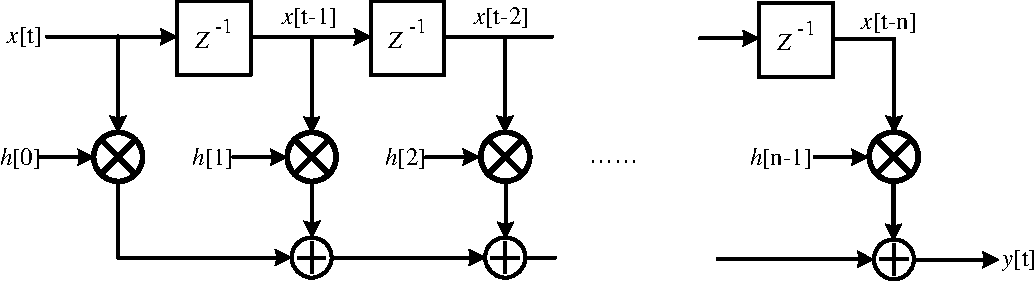
\includegraphics{ellipsoid.files/fir_strctr.pdf}
\caption{img}
\end{figure}

\begin{itemize}
\tightlist
\item
  The time response is: \[y[t] = \sum_{k=0}^{n-1}{h[k]u[t-k]}\]
\end{itemize}

\end{frame}

\begin{frame}{Example: FIR filter design (cont’d)}
\protect\hypertarget{example-fir-filter-design-contd}{}

\begin{itemize}
\item
  The frequency response:
  \[H(\omega)~=~\sum_{m=0}^{n-1}{h(m)e^{-jm\omega}}\]
\item
  The magnitude constraints on frequency domain are expressed as

  \[L(\omega)~\leq~|H(\omega)|~\leq~U(\omega),~\forall~\omega\in(-\infty,+\infty)\]

  where \(L(\omega)\) and \(U(\omega)\) are the lower and upper
  (nonnegative) bounds at frequency \(\omega\) respectively.
\item
  The constraint is non-convex in general.
\end{itemize}

\end{frame}

\begin{frame}{Example: FIR filter design (cont’d)}
\protect\hypertarget{example-fir-filter-design-contd-1}{}

\begin{itemize}
\tightlist
\item
  However, via \emph{spectral factorization}, it can transform into a
  convex one:
  \[L^2(\omega)~\leq~R(\omega)~\leq~U^2(\omega),~\forall~\omega\in(0,\pi)\]
  where

  \begin{itemize}
  \tightlist
  \item
    \(R(\omega)=\sum_{i=-1+n}^{n-1}{r(t)e^{-j{\omega}t}}=|H(\omega)|^2\)
  \item
    \(\mathbf{r}=(r(-n+1),r(-n+2),...,r(n-1))\) are the autocorrelation
    coefficients.
  \end{itemize}
\end{itemize}

\end{frame}

\begin{frame}{Example: FIR filter design (cont’d)}
\protect\hypertarget{example-fir-filter-design-contd-2}{}

\begin{itemize}
\item
  \(\mathbf{r}\) can be determined by \(\mathbf{h}\):

  \[r(t)~=~\sum_{i=-n+1}^{n-1}{h(i)h(i+t)},~t\in\mathbf{Z}.\]

  where \(h(t)=0\) for \(t < 0\) or \(t > n - 1\).
\item
  The whole problem can be formulated as:
\end{itemize}

\[\begin{array}{ll}
  \text{min}  & \gamma \\
  \text{s.t.} & L^2(\omega) \leq R(\omega) \leq U^2(\omega), \; \forall \omega \in [0,\pi]   \\
              & R(\omega) > 0, \forall \omega \in [0,\pi]
\end{array}\]

\end{frame}

\begin{frame}{Experiment}
\protect\hypertarget{experiment}{}

\begin{figure}
\centering
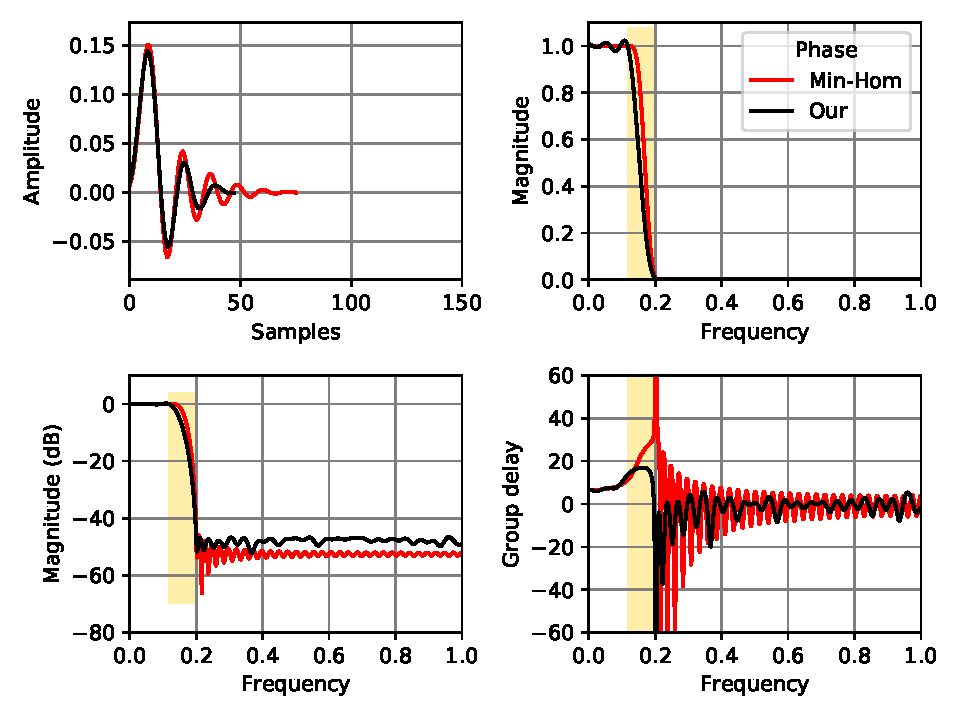
\includegraphics[width=0.5\textwidth,height=\textheight]{ellipsoid.files/lowpass.pdf}
\caption{Result}
\end{figure}

\end{frame}

\begin{frame}{Example: Maximum Likelihood estimation}
\protect\hypertarget{example-maximum-likelihood-estimation}{}

\[\begin{array}{ll}
      \min_{\color{blue}\kappa, p}   &      \log \det (\Omega({\color{blue}p}) + {\color{blue}\kappa}
       \cdot I) + \mathrm{Tr}((\Omega({\color{blue}p}) + {\color{blue}\kappa} \cdot I)^{-1}Y) \\\\
      \text{s.t.} & \Omega({\color{blue}p}) {\color{red}\succeq} 0, {\color{blue}\kappa} {\color{red}\geq} 0 \\\\
 \end{array}\]

Note: the 1st term is concave, the 2nd term is convex

\begin{itemize}
\tightlist
\item
  However, if there are enough samples such that \(Y\) is a positive
  definite matrix, then the function is convex within \([0, 2Y]\)
\end{itemize}

\end{frame}

\begin{frame}{Example: Maximum Likelihood estimation (cont’d)}
\protect\hypertarget{example-maximum-likelihood-estimation-contd}{}

\begin{itemize}
\tightlist
\item
  Therefore, the following problem is convex:
\end{itemize}

\[\begin{array}{ll}
      \min_{\color{blue}\kappa, p}   &   \log \det V({\color{blue}p}) + \mathrm{Tr}(V({\color{blue}p})^{-1}Y) \\\\
      \text{s.t.} & \Omega({\color{blue}p}) + {\color{blue}\kappa} \cdot I = V({\color{blue}p}) \\\\
                    & 0 \preceq V({\color{blue}p}) \preceq 2Y, {\color{blue}\kappa} {>} 0
\end{array}\]

\end{frame}

\hypertarget{discrete-optimization}{%
\section{Discrete Optimization}\label{discrete-optimization}}

\begin{frame}{Why Discrete Convex Programming}
\protect\hypertarget{why-discrete-convex-programming}{}

\begin{itemize}
\item
  Many engineering problems can be formulated as a convex/geometric
  programming, e.g.~digital circuit sizing
\item
  Yet in an ASIC design, often there is only a limited set of choices
  from the cell library. In other words, some design variables are
  discrete.
\item
  The discrete version can be formulated as a Mixed-Integer Convex
  programming (MICP) by mapping the design variables to integers.
\end{itemize}

\end{frame}

\begin{frame}{What’s Wrong w/ Existing Methods?}
\protect\hypertarget{whats-wrong-w-existing-methods}{}

\begin{itemize}
\item
  Mostly based on relaxation.
\item
  Then use the relaxed solution as a lower bound and use the
  branch–and–bound method for the discrete optimal solution.

  \begin{itemize}
  \tightlist
  \item
    Note: the branch-and-bound method does not utilize the convexity of
    the problem.
  \end{itemize}
\item
  What if I can only evaluate constraints on discrete data? Workaround:
  convex fitting?
\end{itemize}

\end{frame}

\begin{frame}{Mixed-Integer Convex Programming}
\protect\hypertarget{mixed-integer-convex-programming}{}

Consider: \[\begin{array}{ll}
        \text{minimize}      & f_0(x), \\
        \text{subject to}    & f_j(x) \leq 0, \; \forall j=1,2,\ldots \\
                             & x \in \mathbb{D} 
\end{array}\]

where

\begin{itemize}
\tightlist
\item
  \(f_0(x)\) and \(f_j(x)\) are “convex”
\item
  Some design variables are discrete.
\end{itemize}

\end{frame}

\begin{frame}{Oracle Requirement}
\protect\hypertarget{oracle-requirement}{}

\begin{itemize}
\item
  The oracle looks for the nearby discrete solution \(x_d\) of \(x_c\)
  with the cutting-plane:
  \[g^\top (x - x_d) + \beta \leq 0, \beta \geq 0, g \neq 0\]
\item
  Note: the cut may be a shallow cut.
\item
  Suggestion: use different cuts as possible for each iteration (
  e.g.~round-robin the evaluation of constraints)
\end{itemize}

\end{frame}

\begin{frame}{Example: FIR filter design}
\protect\hypertarget{example-fir-filter-design-1}{}

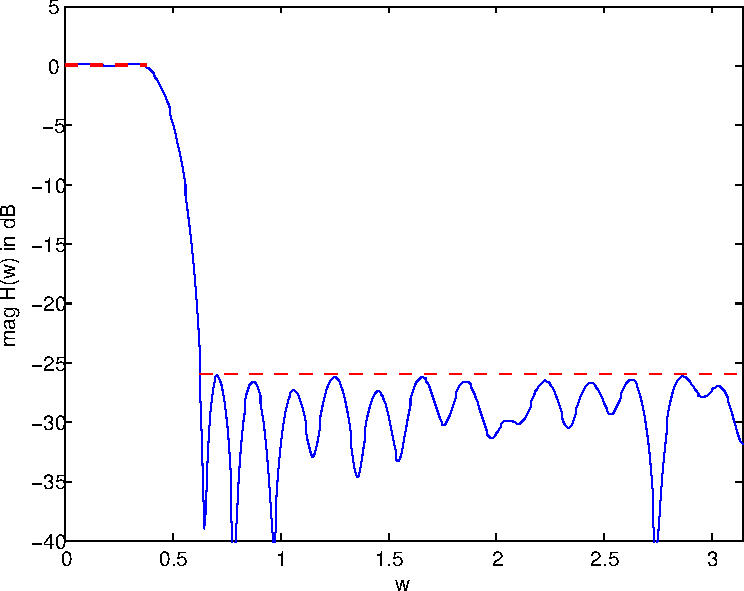
\includegraphics[width=0.9\textwidth,height=\textheight]{ellipsoid.files/lowpass_ripple.pdf}

\end{frame}

\hypertarget{q-a}{%
\section{Q \& A}\label{q-a}}

\end{document}
